\chapter*{Research Papers}
\begin{small}
\begin{enumerate}[label=\numberingI{\textbf{P\arabic*}}]
    \item Gianni, Francesco, and Monica Divitini (2016) \textbf{\enquote{Technology-Enhanced Smart City Learning: A Systematic Mapping of the Literature.}} \emph{Interaction Design and Architecture(s) Journal - IxD\&A} 27:28--43.
    
    \item Mora, Simone, Francesco Gianni, and Monica Divitini (2017) \textbf{\enquote{Tiles: A Card-Based Ideation Toolkit for the Internet of Things.}} In: Proceedings of the 2017 Conference on Designing Interactive Systems. DIS 2017. 587--598. Edinburgh, United Kingdom: ACM.
    
    \item Gianni, Francesco, and Monica Divitini (2018) \textbf{\enquote{Designing IoT Applications for Smart Cities: Extending the Tiles Ideation Toolkit.}} \emph{Interaction Design and Architecture(s) Journal - IxD\&A} 35:100--116.
    
    \item Gianni, Francesco, Lisa Klecha, and Monica Divitini (2019) \textbf{\enquote{Tiles-Reflection: Designing for Reflective Learning and Change Behaviour in the Smart City.}} In: The Interplay of Data, Technology, Place and People for Smart Learning. SLERD 2018. \emph{Smart Innovation, Systems and Technologies} 95:70--82. Aalborg, Denmark: Springer, Cham.
   
    \item Mavroudi, Anna, Monica Divitini, Francesco Gianni, Simone Mora and Dag R. Kvittem (2018) \textbf{\enquote{Designing IoT Applications in Lower Secondary Schools.}} In: Proceedings of IEEE Global Engineering Education Conference. EDUCON 2018. 1120--1126. Tenerife, Spain: IEEE.
    
    \item Gianni, Francesco, Simone Mora, and Monica Divitini (2018) \textbf{\enquote{RapIoT Toolkit: Rapid Prototyping of Collaborative Internet of Things Applications.}} \emph{Journal of Future Generation Computer Systems.} Elsevier.
    
    \item Gianni, Francesco, Simone Mora, and Monica Divitini (2018) \textbf{\enquote{Rapid Prototyping Internet of Things Applications for Augmented Objects: The Tiles Toolkit Approach.}} In: Ambient Intelligence. AmI 2018. \emph{Lectures Notes in Computer Science.} 11249:204--220. Larnaca, Cyprus: Springer, Cham.
\end{enumerate}
\end{small}

%PAPER 1
\cleardoublepage
\begin{flushright}
\textsc{\huge Paper 1}
\end{flushright}
\vspace{3cm}
\begin{center}
	\begin{framed}
		{\Large \textbf{Technology-Enhanced Smart City Learning:\\ A Systematic Mapping of the Literature}}
		
		\medskip
		Francesco Gianni and Monica Divitini
		
		\medskip		
		\emph{Interaction Design and Architecture(s) Journal -- IxD\&A}
	\end{framed}	
\end{center}

\vspace{9cm}


\includegraphics[height=20pt]{by-nc-nd}\\
{\scriptsize Copyright \textcircled{c} 2019. This manuscript version is made available under the \textbf{CC-BY-NC-ND 4.0} license.}\\
{\tiny https://creativecommons.org/licenses/by-nc-nd/4.0/}\\

\includegraphics[height=13pt]{OA} {\scriptsize -- IxD\&A is a Gold Open Access (OA) Journal.}
\cleardoublepage
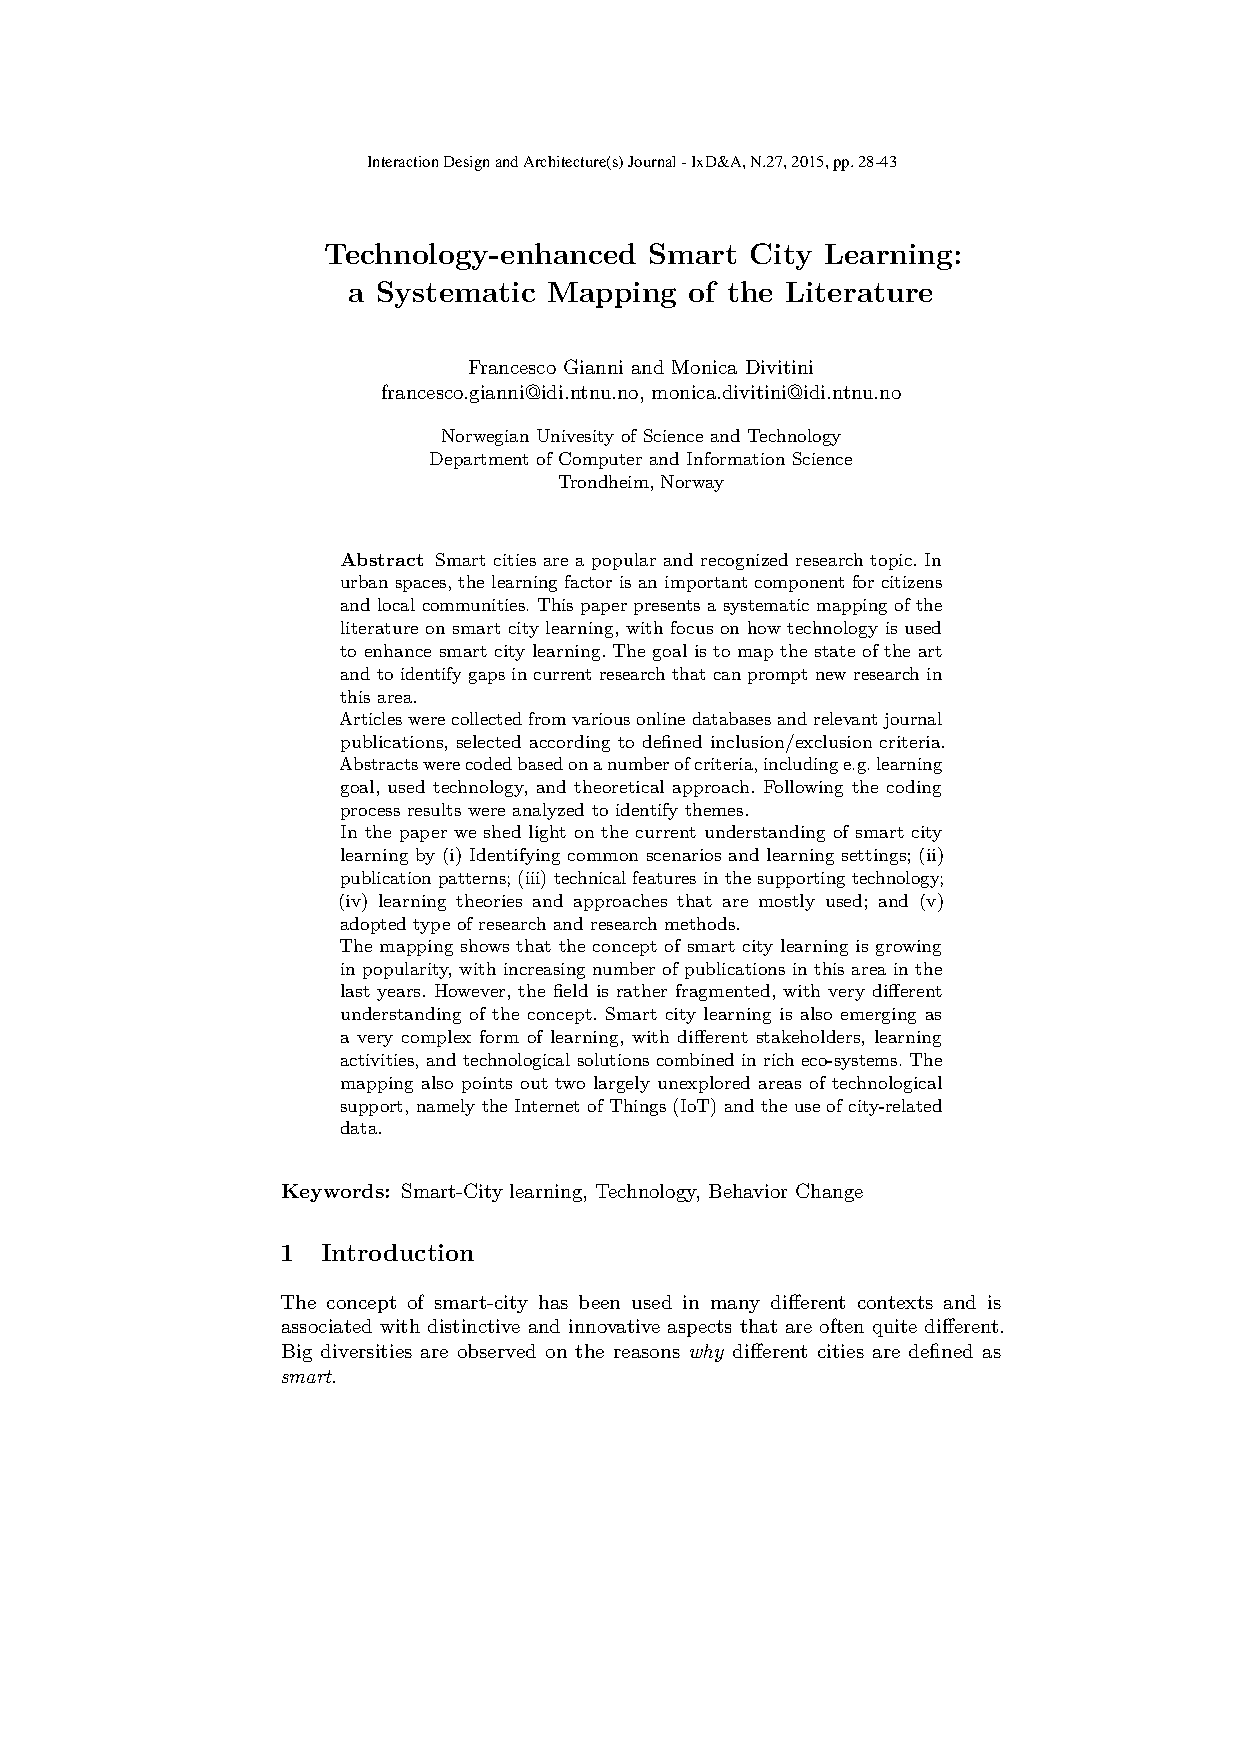
\includepdf[pages=-, noautoscale=true, scale=1, offset=5mm -5mm]{./papers_published/P1.pdf}

%PAPER 2
\cleardoublepage
\begin{flushright}
\textsc{\huge Paper 2}
\end{flushright}
\vspace{3cm}
\begin{center}
	\begin{framed}
		{\Large \textbf{Tiles: A Card-Based Ideation Toolkit\\ for the Internet of Things}}
		
		\medskip
		Simone Mora, Francesco Gianni and Monica Divitini
		
		\medskip		
		\emph{In: Proceedings of the 2017 Conference on Designing Interactive Systems (DIS)}
	\end{framed}
\end{center}

\vspace{10cm}

{\scriptsize Reprinted with kind permission from the Association for Computing Machinery (ACM).}\\
{\tiny DOI: https://doi.org/10.1145/3064663.3064699}
\cleardoublepage
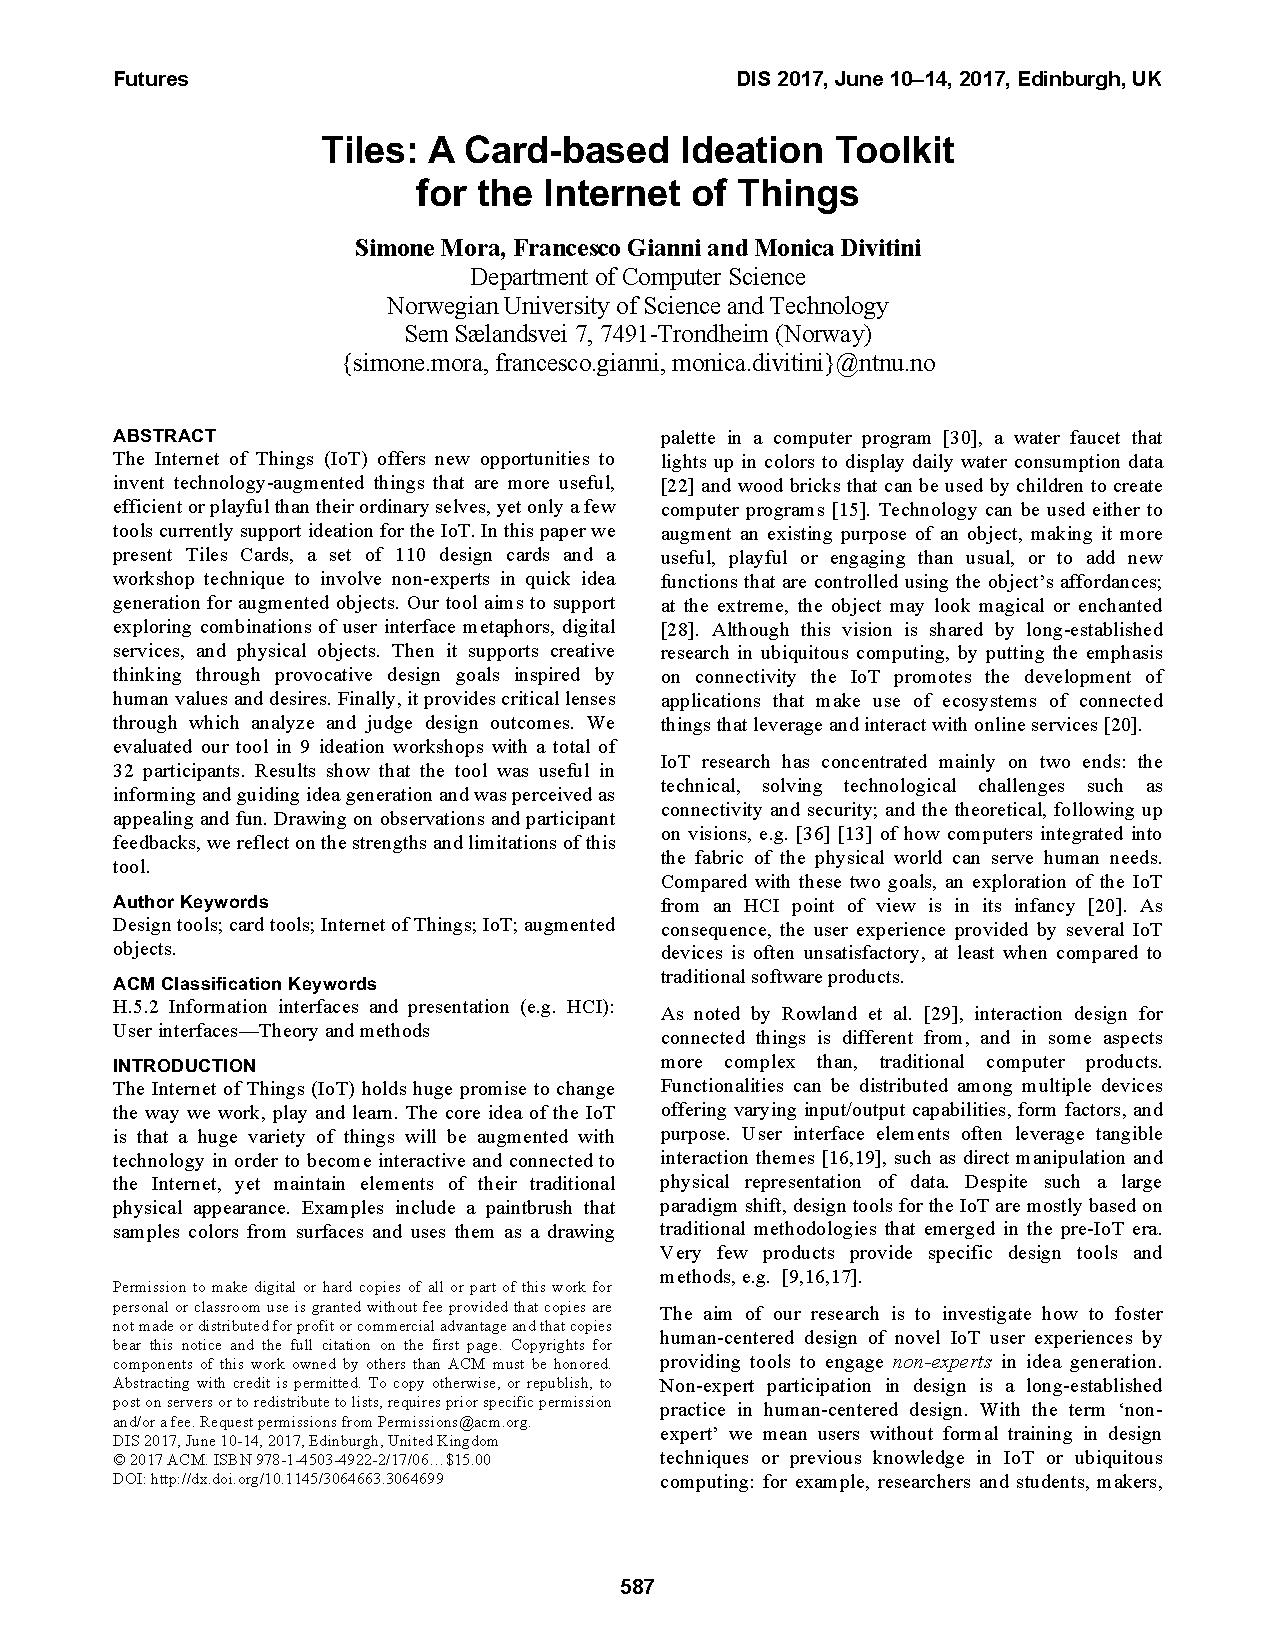
\includepdf[pages=-, noautoscale=true, scale=0.73, offset=5mm 0mm]{./papers_published/P2.pdf}

%PAPER 3
\cleardoublepage
\begin{flushright}
\textsc{\huge Paper 3}
\end{flushright}
\vspace{3cm}
\begin{center}
	\begin{framed}
		{\Large \textbf{Designing IoT Applications for Smart Cities:\\ Extending the Tiles Ideation Toolkit}}
		
		\medskip
		Francesco Gianni and Monica Divitini
		
		\medskip
		\emph{Interaction Design and Architecture(s) Journal -- IxD\&A}
	\end{framed}
\end{center}

\vspace{9cm}


\includegraphics[height=20pt]{by-nc-nd}\\
{\scriptsize Copyright \textcircled{c} 2019. This manuscript version is made available under the \textbf{CC-BY-NC-ND 4.0} license.}\\
{\tiny https://creativecommons.org/licenses/by-nc-nd/4.0/}\\

\includegraphics[height=13pt]{OA} {\scriptsize -- IxD\&A is a Gold Open Access (OA) Journal.}
\cleardoublepage
\includepdf[pages=-, noautoscale=true, scale=1, offset=5mm -5mm]{./papers_published/P3_thesis_edit.pdf}

%PAPER 4
\cleardoublepage
\begin{flushright}
\textsc{\huge Paper 4}
\end{flushright}
\vspace{3cm}
\begin{center}
	\begin{framed}
		{\Large \textbf{Tiles-Reflection: Designing for Reflective Learning and Change Behaviour in the Smart City}}
		
		\medskip
		Francesco Gianni, Lisa Klecha, and Monica Divitini
		
		\medskip
		\emph{In: The Interplay of Data, Technology, Place and People for Smart Learning (SLERD)}
	\end{framed}	
\end{center}

\vspace{10cm}

{\scriptsize Reprinted by permission from Springer International Publishing AG: Springer Nature -- The Interplay of Data, Technology, Place and People for Smart Learning. Knoche H., Popescu E., Cartelli A., {\tiny \textcircled{c} 2019.}}
\cleardoublepage
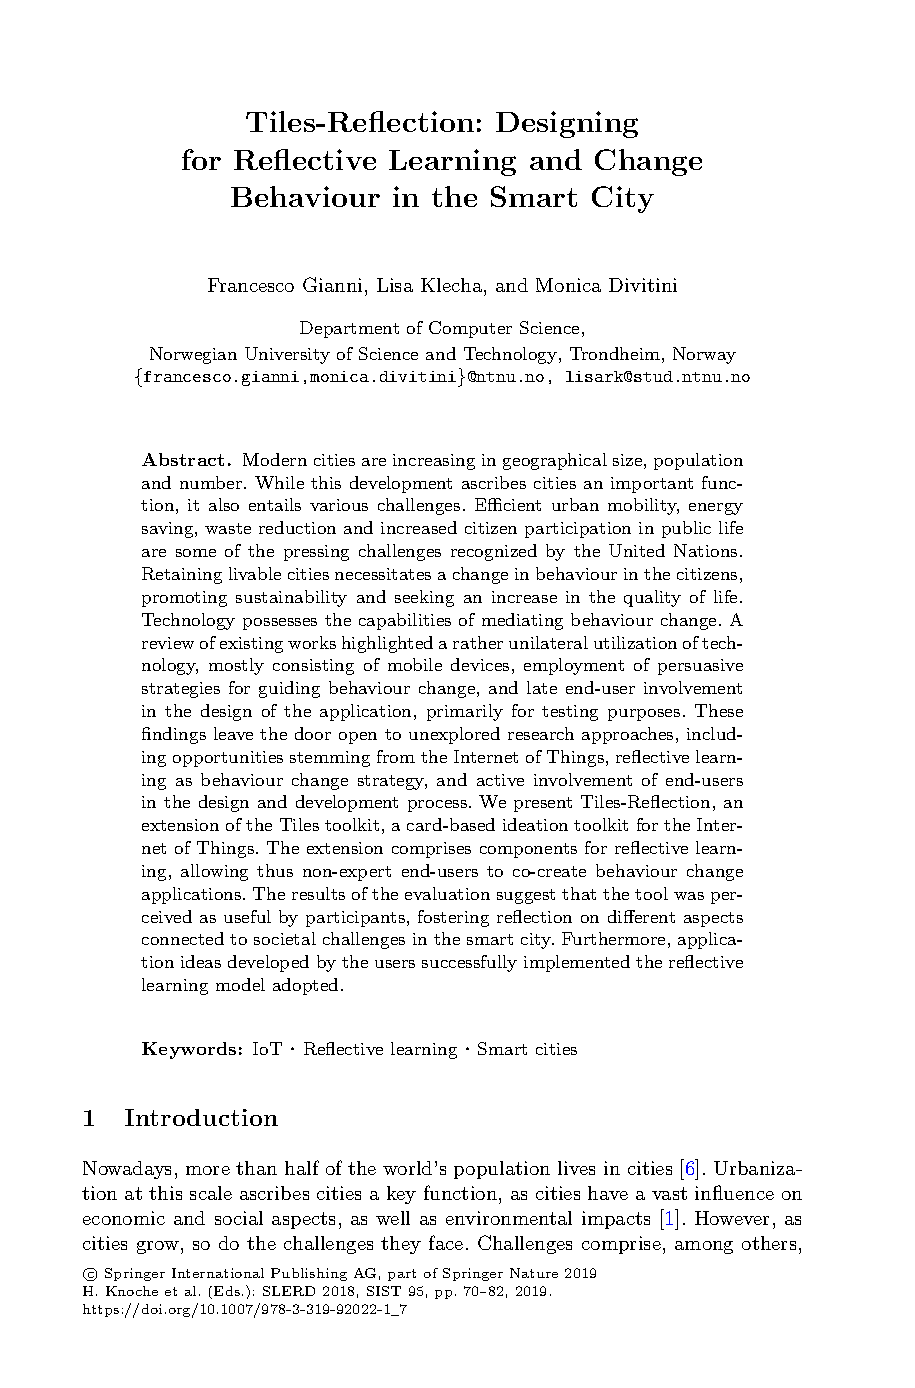
\includepdf[pages=-, noautoscale=true, scale=1, offset=7mm 0mm]{./papers_published/P4_thesis_edit.pdf}


%PAPER 5
\cleardoublepage
\begin{flushright}
\textsc{\huge Paper 5}
\end{flushright}
\vspace{3cm}
\begin{center}
	\begin{framed}
		{\Large \textbf{Designing IoT Applications in Lower Secondary Schools}}
		
		\medskip
		Anna Mavroudi, Monica Divitini, Francesco Gianni,\\ Simone Mora and Dag R. Kvittem
		
		\medskip
		\emph{In: Proceedings of IEEE Global Engineering Education Conference (EDUCON)}
	\end{framed}	
\end{center}

\vspace{9cm}

{\scriptsize \textcircled{c} 2019 IEEE. Reprinted, with permission, from: A. Mavroudi, M. Divitini, F. Gianni, S. Mora and D. R. Kvittem, \enquote{Designing IoT applications in lower secondary schools}, 2018 IEEE Global Engineering Education Conference (EDUCON), Tenerife, 2018, pp. 1120-1126.}\\
{\tiny DOI: https://doi.org/10.1109/EDUCON.2018.8363355}
\cleardoublepage
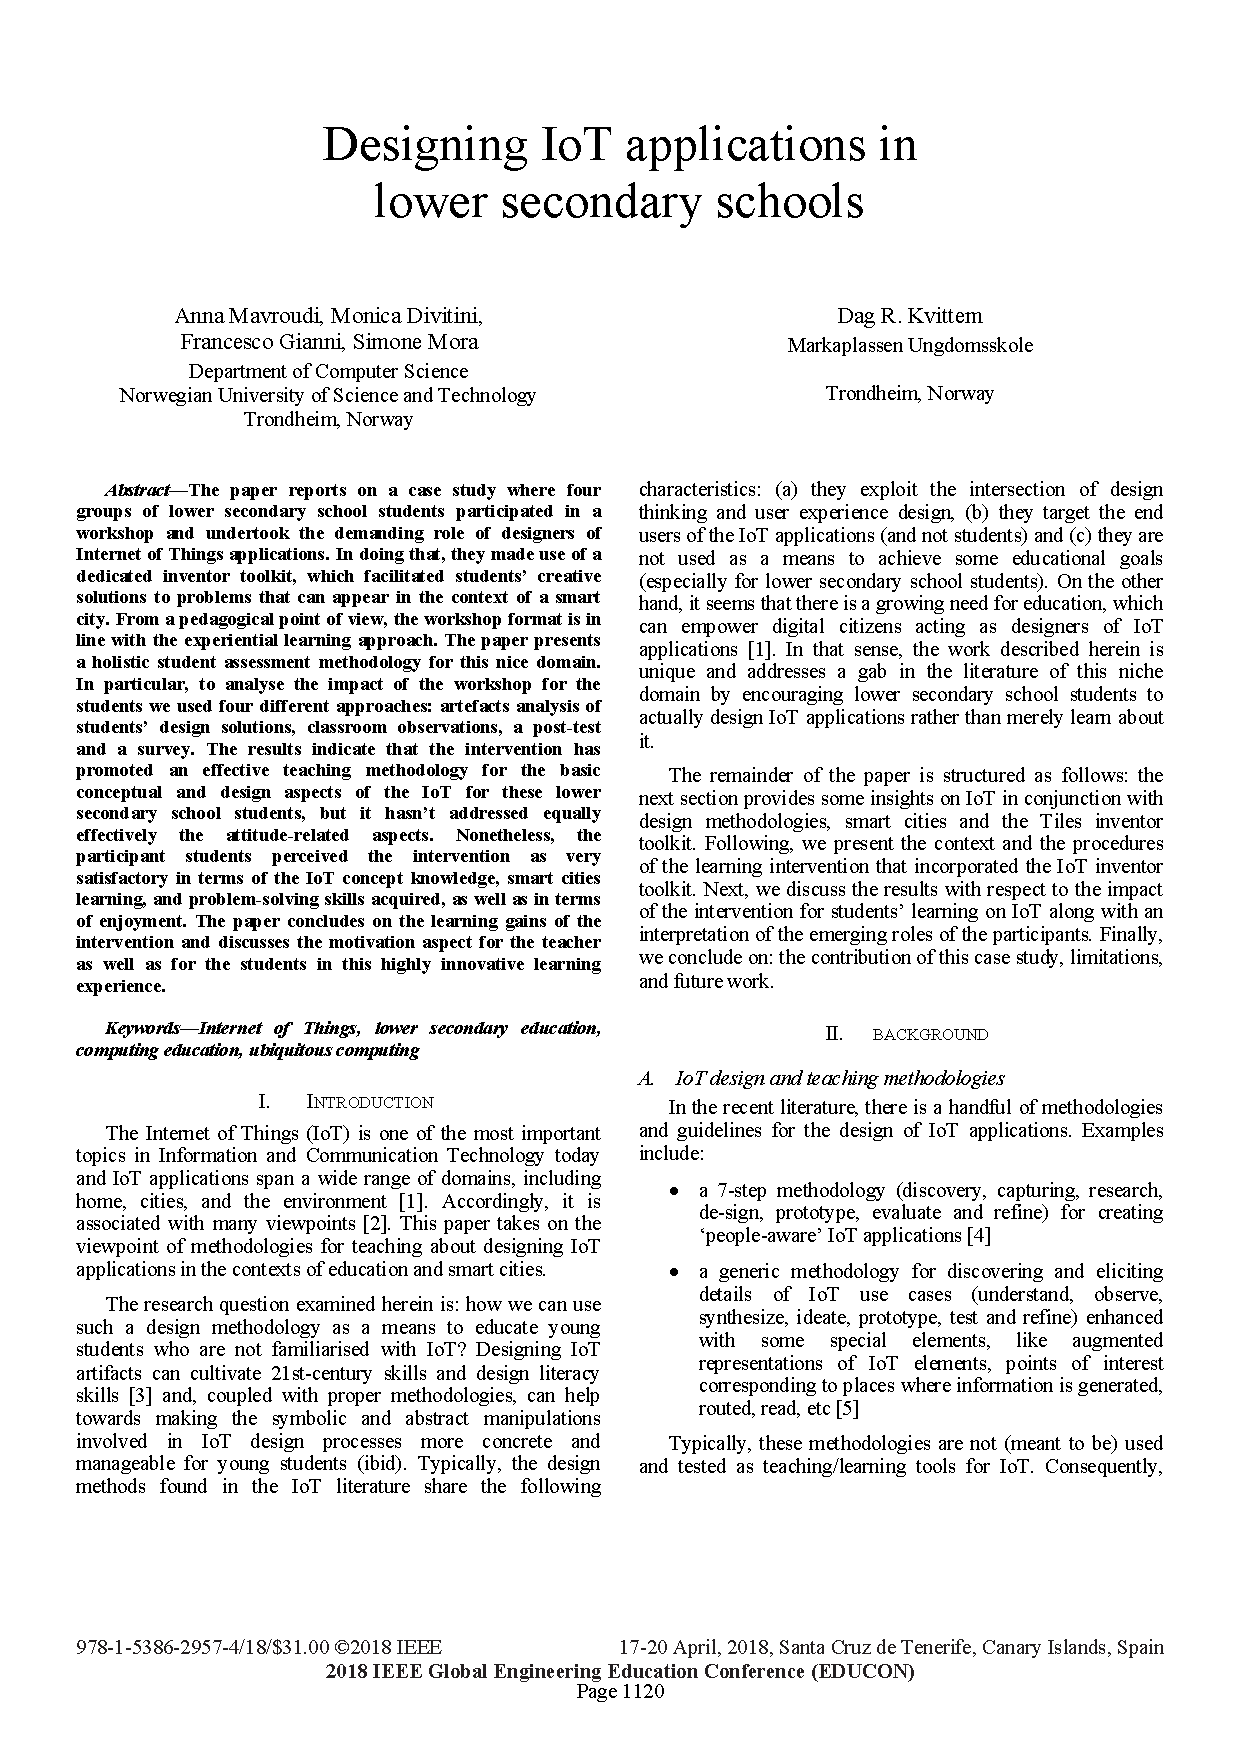
\includepdf[pages=-, noautoscale=true, scale=0.7, offset=6mm 0mm]{./papers_published/P5.pdf}


%PAPER 6
\cleardoublepage
\begin{flushright}
\textsc{\huge Paper 6}
\end{flushright}
\vspace{3cm}
\begin{center}
	\begin{framed}
		{\Large \textbf{RapIoT Toolkit: Rapid Prototyping of Collaborative Internet of Things Applications}}	
		\medskip
		
		Francesco Gianni, Simone Mora, and Monica Divitini
		
		\medskip
		\emph{Journal of Future Generation Computer Systems}
	\end{framed}	
\end{center}

\vspace{10cm}

{\scriptsize \textcircled{c} 2019 Elsevier B.V. Reprinted, with permission, from: F.Gianni, et al., RapIoT toolkit: Rapid prototyping of collaborative Internet of Things applications, Future Generation Computer Systems (2018), https://doi.org/10.1016/j.future.2018.02.030}
\cleardoublepage
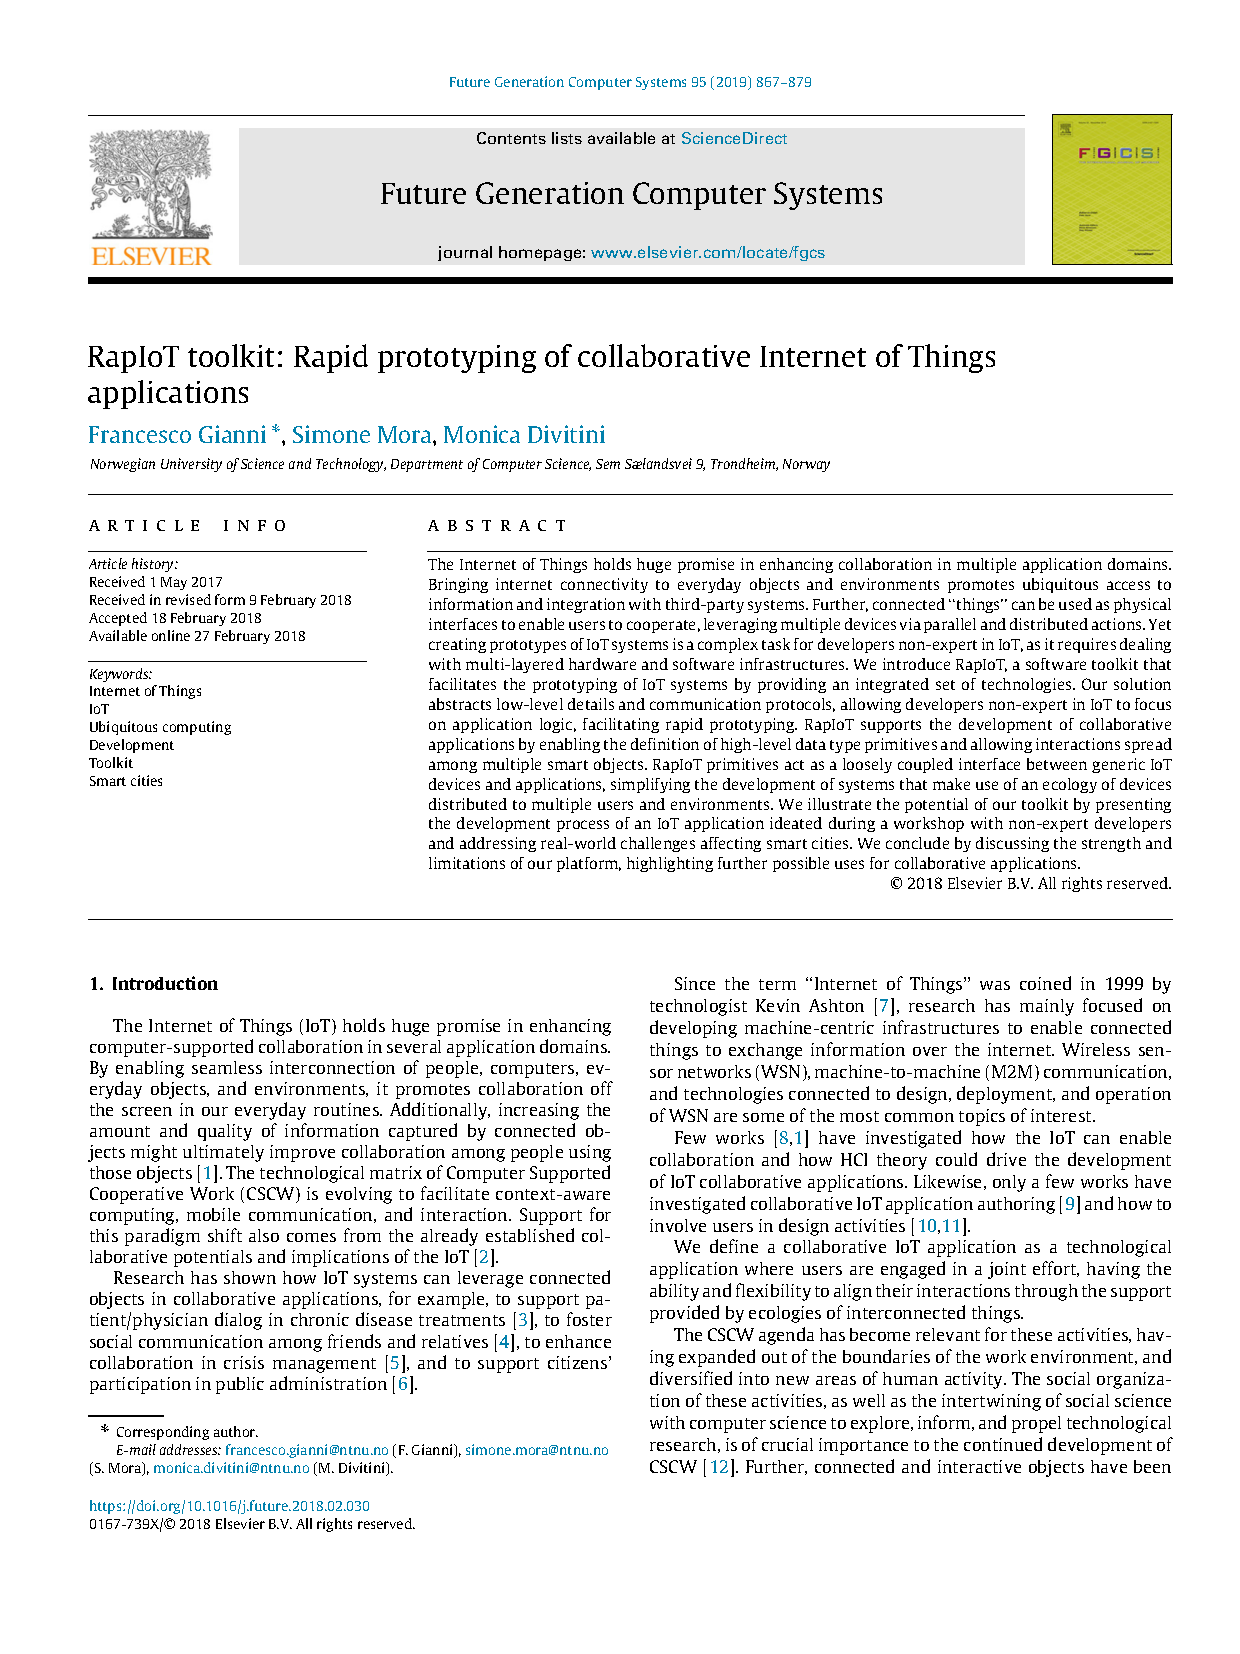
\includepdf[pages=-, noautoscale=true, scale=0.7, offset=5mm 0mm]{./papers_published/P6.pdf}


%PAPER 7
\cleardoublepage
\begin{flushright}
\textsc{\huge Paper 7}
\end{flushright}
\vspace{3cm}
\begin{center}
	\begin{framed}
		{\Large \textbf{Rapid Prototyping Internet of Things Applications for Augmented Objects: The Tiles Toolkit Approach}}	
		\medskip
		
		Francesco Gianni, Simone Mora, and Monica Divitini
		
		\medskip		
		\emph{In: Ambient Intelligence (AmI)}
	\end{framed}	
\end{center}

\vspace{10cm}

{\scriptsize Reprinted by permission from Springer International Publishing AG: Springer Nature -- Ambient Intelligence. Kameas A., Stathis K., \textcircled{c} 2019.}
\cleardoublepage
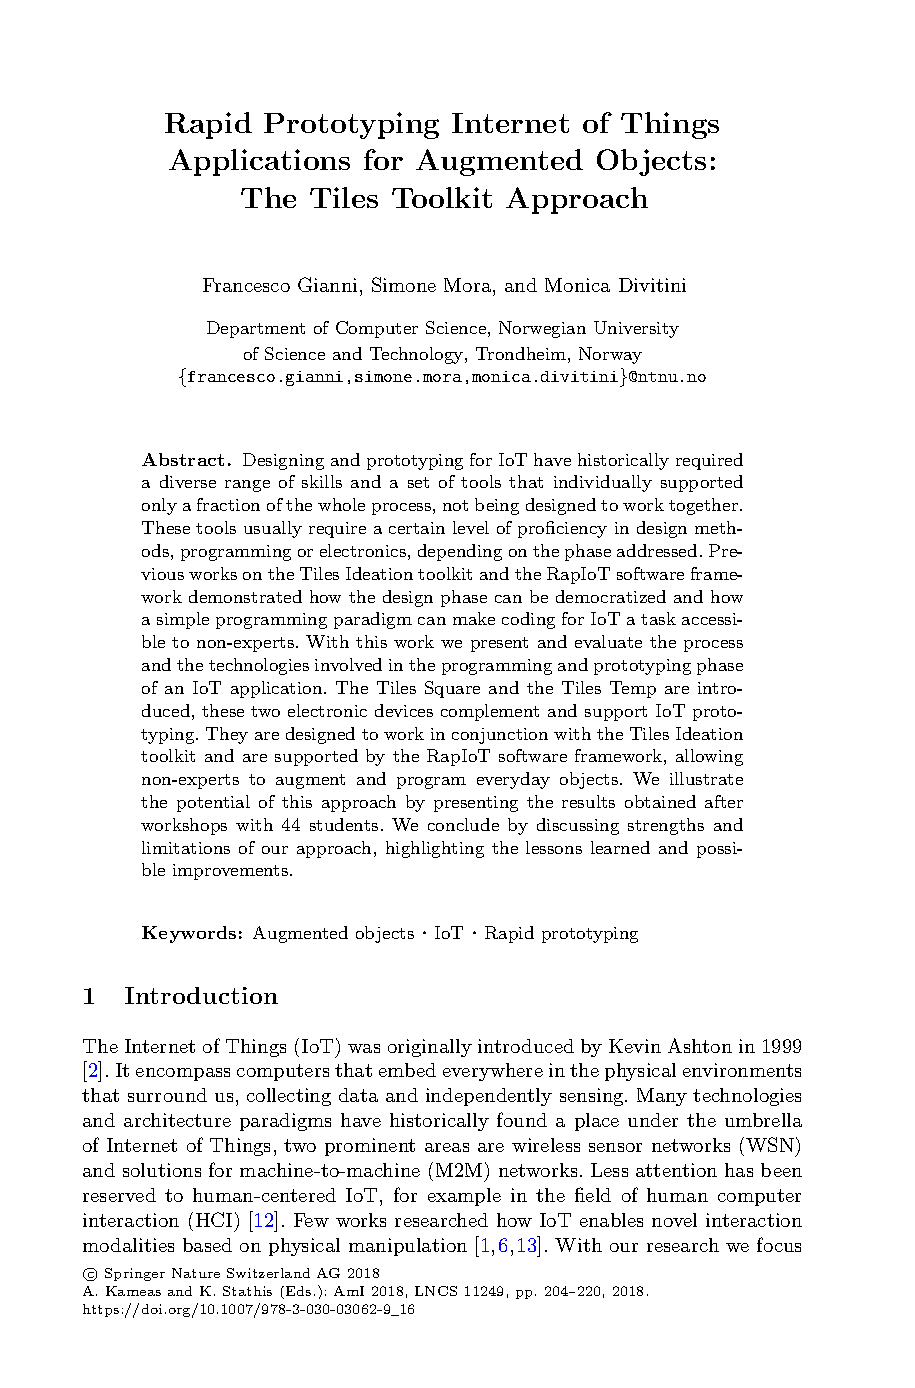
\includepdf[pages=-, noautoscale=true, scale=1, offset=7mm 0mm]{./papers_published/P7_thesis_edit.pdf}
